\documentclass[tikz]{standalone}
\usepackage{pgfplots}
%\pgfplotsset{width=7cm,compat=1.18}
\usepgfplotslibrary{statistics}
\def\axisdefaultwidth{6cm}
\def\axisdefaultheight{6cm}
%\pgfplotsset{every axis/.style={scale only axis}} 		

\begin{document}

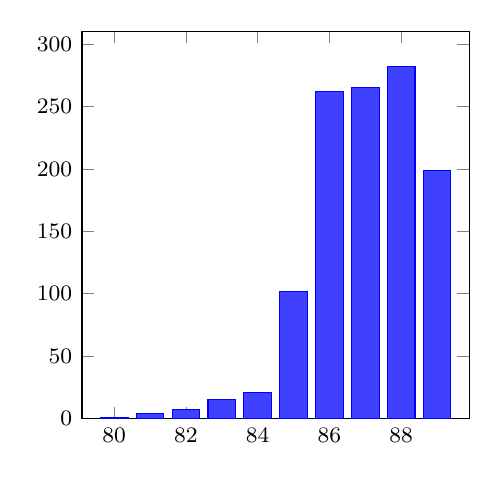
\begin{tikzpicture}
%\begin{axis}[small,ymin=0,title=\texttt{gain (dB)}]
\begin{axis}[small,ymin=0]
\addplot [
ybar,
fill=blue!75,
draw=blue]
table [x=perf, y=cnt] {
cnt                 perf                
1.00000             80.00000            
4.00000             81.00000            
7.00000             82.00000            
15.00000            83.00000            
21.00000            84.00000            
102.00000           85.00000            
262.00000           86.00000            
265.00000           87.00000            
282.00000           88.00000            
199.00000           89.00000            
};
\end{axis}
\end{tikzpicture}
\end{document}
